\section{Background and Motivation}
\label{motivation}

We briefly motivate the potential for dual-technology main memory and the importance of huge pages under virtualized execution.

%\begin{figure}[t]
%\centering
%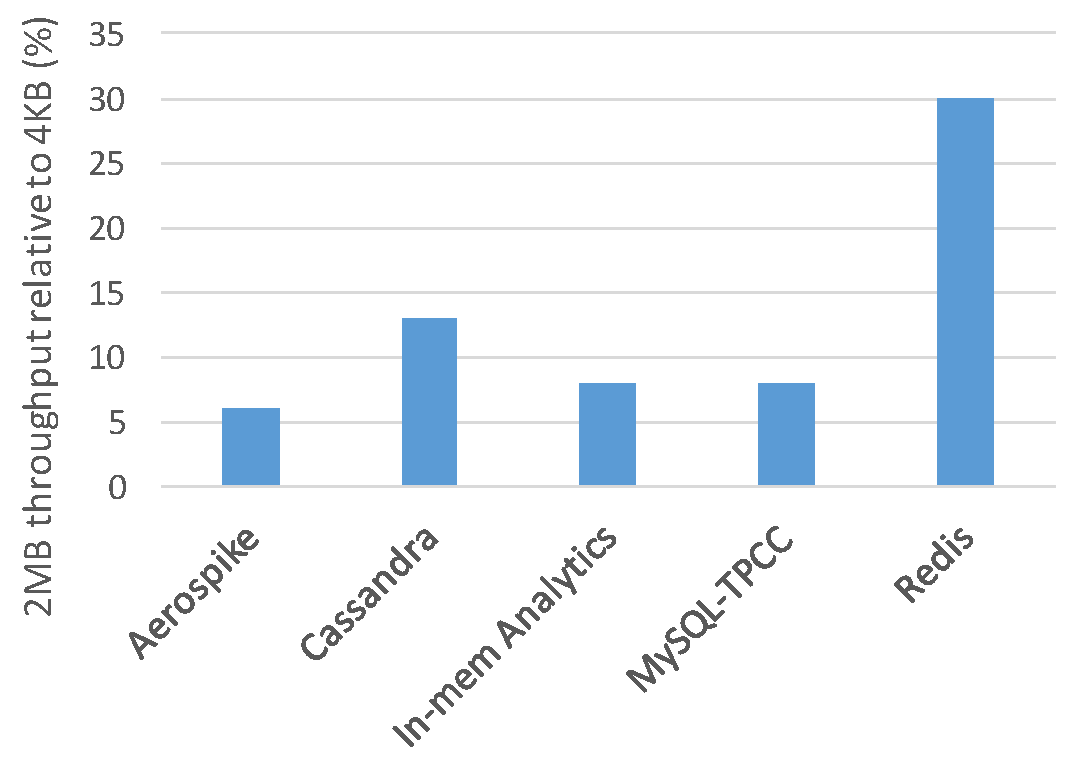
\includegraphics[width=1.0\columnwidth]{figures/thp-perf-improvement.pdf}
%\caption{Throughput improvement by 2MB pages under virtualization relative to
%4KB pages on both host and guest.}
%%\vspace{-0.175in}
%\label{fig:thp-benefit}
%\end{figure}
%

\subsection{Shifting cold data to cheap memory}
\label{analytic-model}

For performance-sensitive and high-footprint cloud applications, it is unlikely that cheaper-but-slower
memory technologies, such as Intel's 3D XPoint memory~\cite{3dcrosspoint}, will 
entirely supplant DRAM main memory.
An increase in memory access latency by even a small multiple (e.g., to 500ns)
will result in drastic throughput losses, as the working set of these applications typically
greatly exceeds cache capacities.
%\fixme{Should we add in a result for slowdown if badger trap traps on every
%page? Neha: not possible, applications stall for very long time durations.}
Because DRAM accounts for only a fraction of total system cost, the net cost of the
throughput loss will greatly outweigh the savings in main memory cost.

However, cloud applications typically have highly skewed access distributions, where
a significant fraction of the application's footprint is infrequently
accessed~\cite{ycsb}.
These rarely accessed pages can be mapped to slow memory without significantly impacting performance.
We refer to this infrequently accessed data as ``cold'' data.

\begin{figure}[t]
\centering
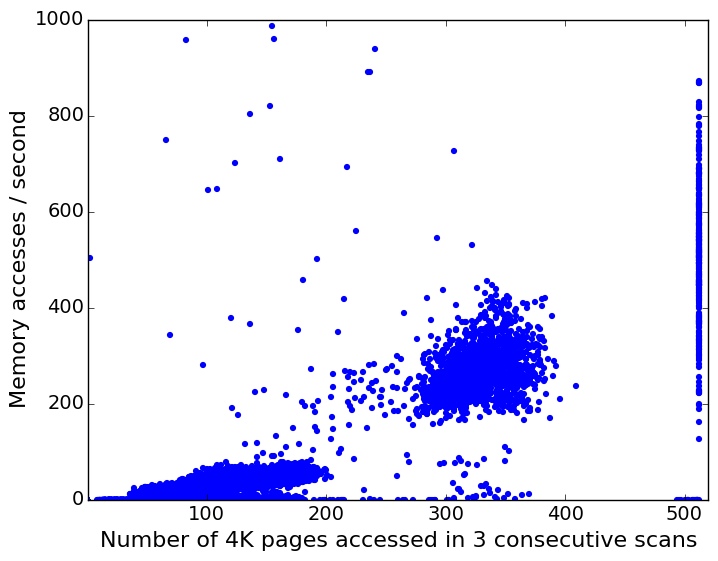
\includegraphics[width=1.0\columnwidth]{asplos2017/figures/redis-plot-3.png}
\caption{Memory access rate vs. hardware {\it Accessed} bit distribution of 4KB
regions within 2MB pages for Redis. The single hardware {\it Accessed} bit per page
does not correlate with memory access rate per page, and thus cannot
estimate page access rates with low overhead.}
\label{fig:redis-access-bit}
\end{figure}

To distinguish cold pages from frequently accessed hot pages, existing
mechanisms exploit the \emph{Accessed} bit in the PTE (set by the hardware each time
the PTE is accessed by a page walk)~\cite{kstaled,vmware-mm,
ref:Guo:2015:PBL:2731186.2731187}. We
investigated one such existing cold-page detection framework, {\tt
kstaled}~\cite{kstaled}. However, we find that the single accessed bit
per page is insufficient to distinguish hot and cold 2MB huge pages with 
sufficiently low overhead. To detect a page access, {\tt kstaled} must clear the
 \emph{Accessed} bit  and flush the corresponding TLB entry.  However, 
 distinguishing hot and cold pages requires monitoring (and hence, clearing)
 accessed bits at high frequency, resulting in unacceptable slowdowns.

Figure~\ref{fig:redis-access-bit} illustrates why hot and cold 2MB huge pages 
cannot be distinguished by temporally sampling
the hardware-maintained access bits at the highest possible rate that can meet
our tight performance degradation target (3\% slowdown), using Redis as an example workload.
The hardware can facilitate 
monitoring at 4KB granularity by temporarily splitting a huge page and monitoring
the accessed bits of the 512 constituent 4KB pages (monitoring at 2MB granularity
without splitting provides even worse hot/cold
differentiation~\cite{ref:Guo:2015:PBL:2731186.2731187}). The horizontal axis 
represents the number of detected ``hot'' 4KB regions
in a given 2MB page when monitoring at the maximum frequency that meets our slowdown target. Here
``hot'' refers to pages that were accessed in three consecutive scan intervals.
The vertical axis represents the ground-truth memory access rate for each 2MB page. 
(We describe our methodology for measuring memory access rate in
Section~\ref{section:access-counting}). 
The key take-away is that the scatter plot is highly dispersed---the spatial frequency
of accesses within a 2MB page is poorly correlated with its true access rate.
Conversely, performance constraints preclude monitoring at higher temporal
frequency. Hence, mechanisms that rely solely on {\it Accessed} bit scanning
cannot identify cold pages with low overhead.

%\begin{table}[t]
%\begin{center}
%\begin{tabular}{|c|c|c|c|}
%\hline
%Scan period&Cassandra& MySQL-TPCC &Redis \\
%\hline
%20 sec& 8\% & 10\% & 15\%\\
%\hline
%\end{tabular}
%\vspace{0.05in}
%\caption{Loose bound on throughput degradation.}
%\label{table:slowmemapprox}
%\end{center}
%\end{table}
%
%To approximate the performance impact of migrating such cold pages to slow memory,
%we develop a loose bound on throughput impact by the following simple analysis. Using the \texttt{kstaled} framework,
%we can measure the number of pages that are not accessed during a given time
%duration. Suppose $P$ pages are not accessed for a time duration $T$. Then,
%we can expect that the access rate to each page in $P$ is $\leq 1/T$ 
%%\fixme{I'm not sure this math follows. We need to talk about this more.}. 
%Now,
%assuming that we place the $P$ pages in slow memory, and that each slow
%memory reference has a latency of $t_{slow}$, we can see that the {\it extra}
%time required for accessing slow memory $\leq t_{slow}P/T$. Thus, the benchmark
%throughput will be degraded by $\leq t_{slow}P/T$. In
%Table~\ref{table:slowmemapprox} we show the value of this rough bound on
%throughput degradation.
%
%From Table~\ref{table:slowmemapprox} we can see that for $T = 20s$, i.e.,
%placing all pages that are cold for 20s into slow memory, the performance
%degradation is $\leq 15\%$. Note that our model is conservative, since it
%doesn't consider that many of the detected ``cold'' pages are, in fact, idle for
%even longer periods and have much lower access frequencies than
%$1/T$.
%Nevertheless, this analysis suggests that a large fraction of
%the application footprint can be migrated to slow memory in cloud workloads. In fact, as we
%show in the remainder of this paper, the actual performance impact on the
%application performance is much lower than the simple analytical model predicts
%($\leq 5\%$ for MySQL and Cassandra, and $\leq 10\%$ for Redis).
%
\subsection{Benefits of transparent huge pages}
Intel's IA-64 x86 architecture mandates a 4-level page table structure for 4KB
memory pages.  So, a TLB miss may incur up to four memory accesses to walk the page table. 
Under virtualization, with two-dimensional page table walks (implemented in Intel's
Extended Page Tables and AMD's Nested Page Tables), the cost of a page walk can be as high as
24 memory accesses~\cite{Intel-sw-manual, AMD-NPT}.  When memory is mapped to a 2MB 
huge page in both the guest and host, the worst-case page walk is reduced to 15 accesses, which 
significantly lowers the performance overhead of virtualization. Moreover,
2MB huge pages increase the TLB reach and improve the cacheability of intermediate
levels of the page tables, as fewer total entries compete for cache capacity. 

Table~\ref{tab:thp-benefit} shows the performance benefit of using huge pages
via Linux's Transparent Huge Page (THP) mechanism. We compare throughput of
various cloud applications where both the guest and host employ 2MB huge pages
against configurations with transparent huge pages disabled (i.e., all pages are
4KB). We observe significant throughput benefits as high as 30\% for Redis.
Previous literature has also reported performance benefits of huge
pages~\cite{ref:Guo:2015:PBL:2731186.2731187, Basu2013, hugepages}. From these
results, it is clear that huge pages are essential to performance, and any
attempt to employ a dual-technology main memory must preserve the performance
advantages of huge pages. For this reason, we only evaluate Thermostat with THP
enabled at both host and guest.

%\subsection{Identifying cold data is hard}
%Identifying cold data in applications has been a challenging problem, more so in
%the case where cold data becomes hot later on the application run time. Linux
%kernel developers have built cold data detection mechanisms at run time for any
%given page size granularity ~\cite{kstaled, vmware-mm}. However, those
%mechanisms cannot be used to detect what we call hotspot 4KB pages in otherwise
%cold pages in the applications at run time. Figure~\ref{fig:motivation} shows
%percentage of application data that remains untouched for 20 sec time duration
%at 4KB and 2MB granularity~\footnote{Note that in ARM based architectures huge
%size can be as low as 64KB. However, due to prevalence of x86 based server chips
%we experimented with x86 based machines only.}. Fraction of cold data decreases
%from 50\% to only 20\% as page size granularity is increased from 4KB to 2MB.
%For employing cheaper but slower memory we want large fraction of application
%data to be cold so as to minimize the rate of slow memory access. When using 2MB
%pages there is an opportunity to detect larger fraction of cold data in
%applications that current mechanisms fail to identify. 

%\subsection{Previous techniques are inadequate}
%Why are previous 2-level memory techniques inadequate in solving this issue.
%
%Re-iterate the problem we are solving and the central idea of our solution.
